\documentclass[]{article}

\begin{document}

\section{Functionaliteit}
\label{Functionaliteit}
Alle features die we wilden implementeren zijn ge\"implementeerd. Alle noden van de opdrachtgever (Sectie \ref{Noden}) zijn ge\"implementeerd. Er zijn verschillende uitbreidingen die we toch graag ge\"implementeerd hadden, echter zijn deze features geen core functionaliteit. Deze features zijn niet ge\"implementeerd omwille van zowel tijdsbeperkings als de voorkeur om het programma zorgvoldig af te werken. Deze features worden besproken in Sectie~\ref{uitbreidingen}. \\\\
Eerst worden de verschillende features opgesomd, hierna volgt een meer gedetailleerde beschrijving van de features.

\subsection{Features:}
\begin{itemize}
\item professioneel uiterlijk (neutrale kleuring)
\item beschikbaar in meerdere talen
\item debug modus: stappen doorheen het programma
\item inladen en opslaan van programma's in een leesbaar formaat
\item events aanmaken
\item klassen aanmaken
\item programma opbouwen via blokken
\item blokken verwijderen
\item instanties maken
\item programma uitvoeren
\end{itemize}

\subsection{Extra Features:}
\begin{itemize}
\item selectie plaatsing blokken
\item breakpoints plaatsen
\item typechecking
\item sleep blok
\item data editor
\item kostuums opslaan
\item verplaatsen aanknopingspunt wires
\item naam van een klasse aanpassen
\item doorzichtigheid blokken
\item hulp menu
\item event filter
\end{itemize}

\subsection{Uitleg eatures: }
\subsubsection{Professionele look}
De IDE heeft een \textbf{professioneel} uiterlijk zoals te zien in Figuur~\ref{prof}. De verschillende blokken die de gebruiker kan plaatsen hebben neutrale kleuren. 
\begin{figure}[H]
\centering
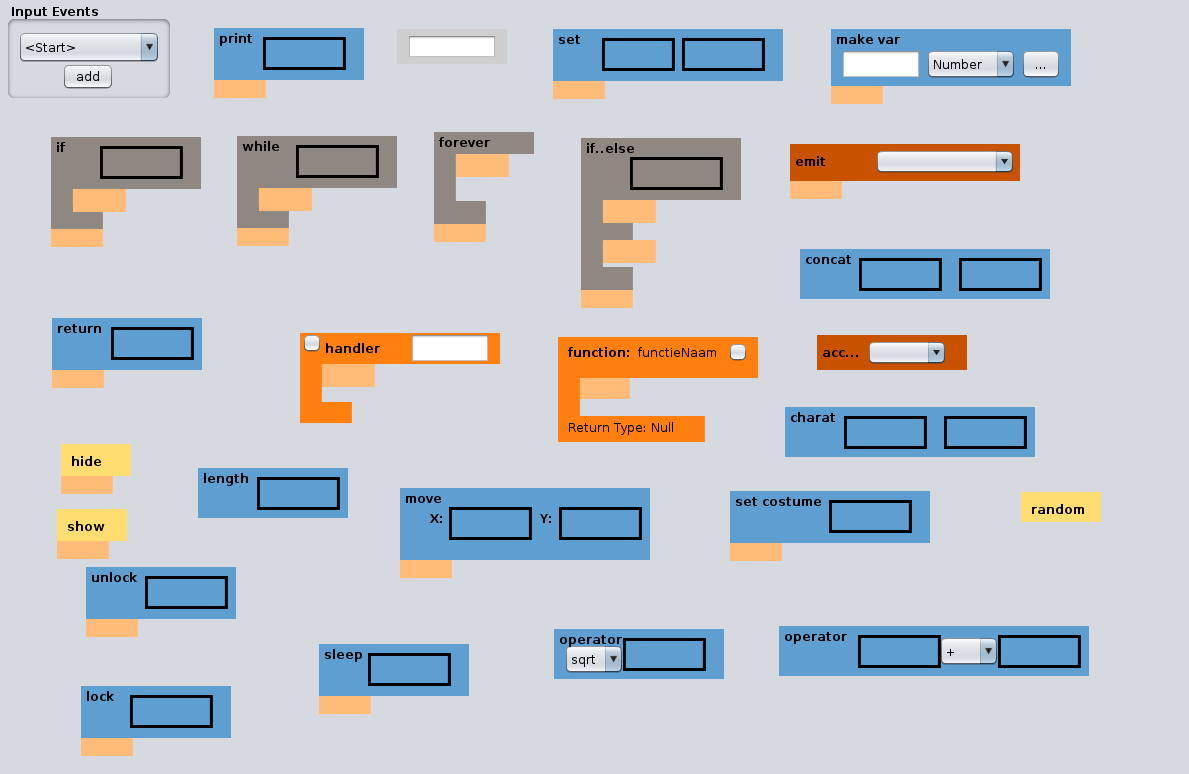
\includegraphics[width=1.1\textwidth]{./Functionaliteit/blocks.png}
\caption{Alle ge\"implementeerde blokken.}
\label{prof}
\end{figure}

\subsubsection{Meerdere talen}
De IDE is beschikbaar in zowel het \textbf{Nederlands als het Engels}. Hoe het wisselen tussen de verschillende talen gebeurt is te zien in Figuur~\ref{lang}
\begin{figure}[H]
\centering
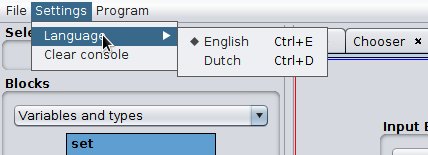
\includegraphics[width=1.1\textwidth]{./Functionaliteit/lang.png}
\caption{Selecteer de taal.}
\label{lang}
\end{figure}

\subsubsection{Inladen en opslaan}
De gebruiker kan programma's \textbf{opslaan en inladen} in een leesbaar formaat, dit gebeurt door middel van het XML-formaat. Het inladen zal de IDE niet doen crashen op een verkeerde layout, er kan wel een eigen error message uitgeprint worden naar de console zodanig dat de gebruiker weet wat er fout gaat. Er is ook de mogelijkheid om een nieuw project te starten, dit verwijdert alle hudige niet opgeslagen progressie.

\subsubsection{Debug modus}
Er is een \textbf{debug modus} aanwezig. Deze laat toe om stap voor stap doorheen het programma te lopen. Er zijn verschillende extra features ge\"implementeerd met betrekking tot de debug modus, deze staan uitgelegd in Sectie~\ref{extra}.
\subsubsection{Events}
De gebruiker kan nieuwe \textbf{events aanmaken en verwijderen}. De inhoud van deze events kan de gebruiker aanpassen. Hij kan nieuwe informatie toevoegen, informatie verwijderen of het type van de informatie aanpassen.

\subsubsection{Klassen}
Klassen kunnen aangemaakt en verwijderd worden.

\subsubsection{Blokken plaatsen}
Het Klasse-view laat toe om \textbf{blokken} te plaatsen. Deze blokken kunnen aan de linkerkant geselecteerd worden. In het dropdown menu staan verschillende categorie\"een met verschillende blokken. Blokken kunnen vervolgens volgens hun regels genest worden in elkaar. Het blokje ``Input Events'' toont alle input events van een bepaalde klasse. Via het dropdown menu kunnen input events toegevoegd worden, via het kruisje kan dat input-event verwijderd worden. Globale variabelen zijn niet toegelaten in de IDE. De gebruiker kan nieuwe member \textbf{variabelen} aanmaken. Een member variabele kan overal in een klasse gebruikt worden. Elke instantie heeft zijn eigen instanties van de member variabelen. Er kunnen verschillende \textbf{kostuums} toegevoegd worden aan een klasse. Deze kan als primair gezet worden, zodanig dat elke instantie van een klasse begint met dat kostuum.

\subsubsection{Blokken verwijderen}
De gebruiker kan een \textbf{blok verwijderen} door middel van een optie die tevoorschijn komt via een popup. Deze popup kan getoond worden als de gebruiker de rechtmuisknop indrukt. De gebruiker kan geen geneste blokken apart verwijderen. Het verwijderen van een blok zal altijd van toepassing zijn op de meest externe blok, deze verwijdert dan ook alle geneste blokken. De reden dat geneste blokken niet verwijderd kunnen worden is duidelijkheid voor de gebruiker. Blokken die genest zijn vormen een geheel. Een actie zoals verwijderen heeft dan ook betrekking op het geheel.

\subsubsection{Instanties}
In het Frame-view kan de gebruiker \textbf{instanties} aanmaken van een Klasse. De gebruiker kan input-events verbinden met output-events van hetzelfde type. Het Canvas-view toont alle instanties en hun geselecteerde uiterlijk. De gebruiker kan deze instanties en verbindingen ook weer verwijderen.

\subsubsection{Uitvoering}
De gebruiker kan een programma \textbf{compileren, uitvoeren, stoppen of stappen} (een stap uitvoeren). Deze actie is mogelijk voor zowel de debug modus als de gewone modus. 

\subsection{Uitleg extra features: }
We hebben verschillende extra features ge\"implementeerd. Sommige features hiervan zijn slechts kleine toevoegingen, andere zijn grotere toevoegingen. 
\label{extra}
\subsubsection{Selecteren blokken}
In zowel het Klasse view als het Frame view kan de gebruiker in de linkerbalk blokken selecteren. Vervolgens zal elke muisklik op het Klasse venster een nieuwe blok van het geselecteerde type maken op de muispositie. Beide views zijn ook ``oneindig'' groot (gelimiteerd door de grote van een int). De blauwe lijn stelt de $x-as$ voor, de rode lijn stelt de $y-as$ voor zoals te zien in Figuur~\ref{infinite}
\begin{figure}[H]
\centering
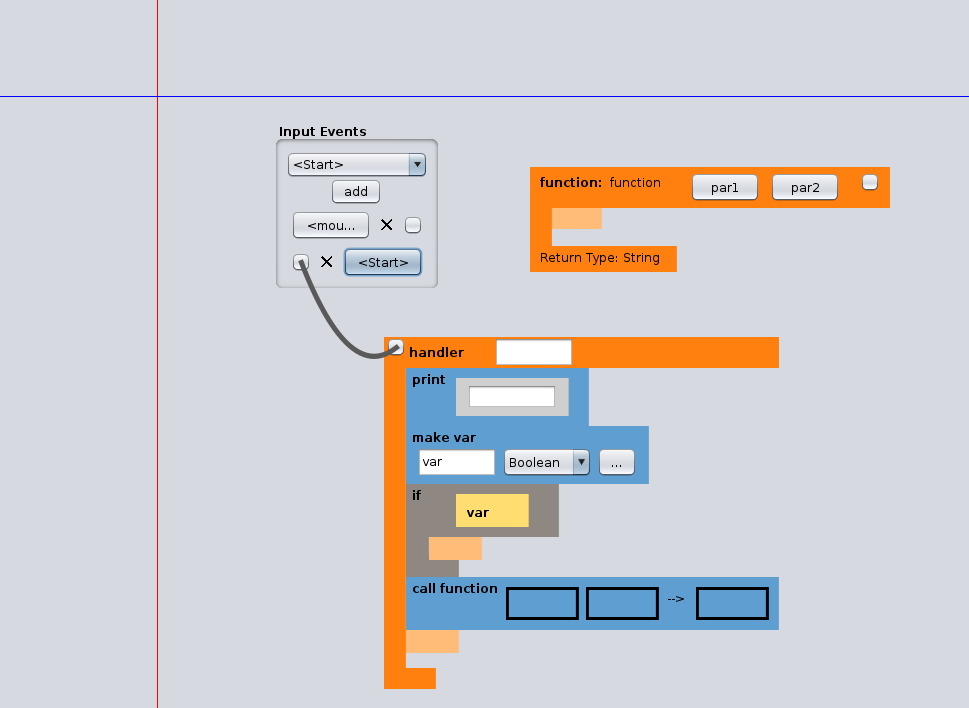
\includegraphics[width=1.1\textwidth]{./Functionaliteit/infinite.png}
\caption{Infinite view}
\label{infinite}
\end{figure}

\subsubsection{Breakpoints plaatsen}
De \textbf{debug modus} is uitgebreid met de mogelijkheid om break-points aan te duiden. Deze kunnen gezet worden op een blok. Als de gebruiker doorheen het programma stapt/loopt in debug modus, gaan zwarte omlijningen aanduiden waar de uitvoer zich momenteel bevindt zoals te zien in Figuur~\ref{debugwindow}. De \texttt{break} stopt enkel het proces dat de \texttt{break} tegenkomt, de andere processen blijven doorlopen.\\\\
\begin{figure}[H]
\centering
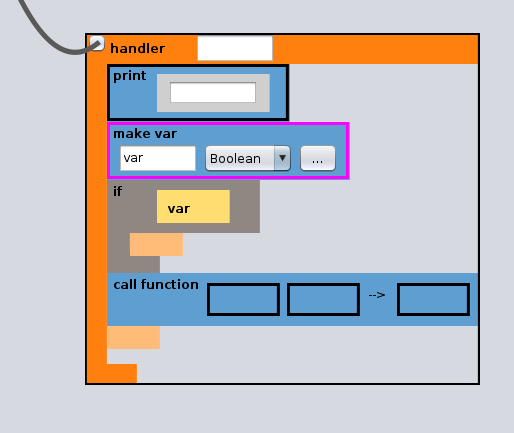
\includegraphics[width=1.1\textwidth]{./Functionaliteit/break.png}
\caption{Debug view}
\label{debugwindow}
\end{figure}

\subsubsection{Typechecking}
Er is ook \textbf{typechecking} toegepast. Dit gebeurt op drie niveau's. Eenderzijds gebeurt typechecking visueel. Dit wordt getoond door een rode border (Sectie~\ref{TypeChecking}). Anderszijds zal de compiler stellen dat compilatie faalt indien het programma niet volledig is. Als er toch fouten door deze checks komen, is er nog runtime errorchecking. Dit kan optreden wanneer een functie aanroep gebeurt naar een niet-bestaande functie. Er wordt dan ook gespecifieerd wat de fout exact is. 

\subsubsection{Sleep blok}
Er is een \texttt{sleep} blok ge\"implementeerd om een proces te laten slapen voor het gespecifieerde aantal milliseconden.

\subsubsection{Data editor}
We hebben een data editor ge\"implementeerd zoals te zien in Figuur~\ref{editor}. De data editor laat het programma zien in zijn XML-vorm. De gebruiker kan deze dan vrij aanpassen. Als de gebruiker terug wisselt naar een ander view zullen de aanpassingen in de data editor ook zichtbaar zijn in de visuele views. De Data editor heeft ook syntax highlighting. Dit is ge\"implementeerd via een externa library \cite{syntax}.
\begin{figure}[H]
\centering
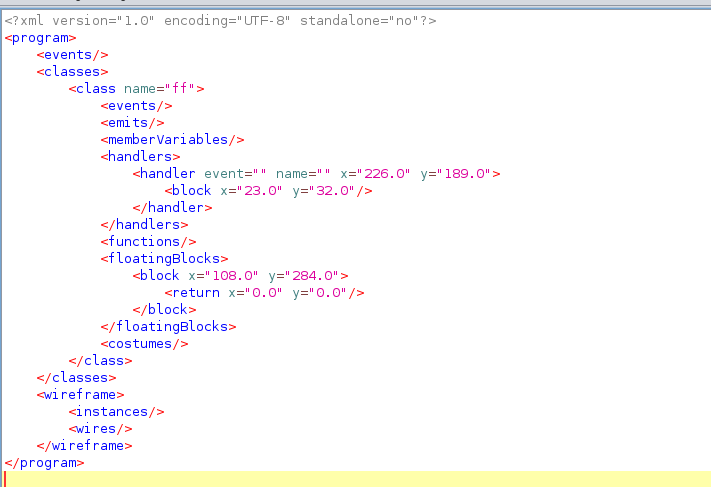
\includegraphics[width=1.1\textwidth]{./Functionaliteit/editor.png}
\caption{Data Editor}
\label{editor}
\end{figure}

\subsubsection{Kostuums opslaan}
De kostuums van een klasse worden ook opgeslagen in dezelfde locatie als de XML-file. Zodanig kan een project gebruikt worden op verschillende computers zonder dat de XML-file aangepast moet worden.

\subsubsection{Aanknopingspunt wire}
Het aanknopingspunt voor een wire kan wisselen van links naar rechts (en andersom) zoals te zien in Figuur~\ref{switchaanknoping}. Dit verhoogt de leesbaarheid bij grotere programma's.
\begin{figure}[H]
\centering
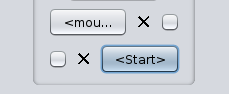
\includegraphics[scale=1]{./Functionaliteit/buttonswitch.png}
\caption{Switchen aanknopingspunt}
\label{switchaanknoping}
\end{figure}

\subsubsection{Naam klasse aanpassen}
De naam van een klasse kan aangepast worden. Door de rechtermuisknop te gebruiken op het tab van die klasse, kan zijn naam aangepast worden. 

\subsubsection{Doorzichtigheid blokken}
Als de gebruiker een blok vast neemt met zijn muis, zal de blok doorzichtig kleuren. Dit maakt het duidelijker voor de gebruiker waar de blok terecht zal komen.

\subsubsection{Hulp menu}
Er is een \textbf{hulp menu} toegevoegd. De gebruiker kan via de rechtermuisknop een hulp-dialoog openen over de blok die zich momenteel onder de muis bevindt. Deze dialoog geeft een korte uitleg over de blok zoals zijn functionaliteit.

\subsubsection{Event filter} 
In het Frame view is een filter ge\"implementeerd. Hierbij kan de zichtbaarheid van events geregeld worden. Verbindingen tussen instanties kunnen op deze manier zichtbaar/onzichtbaar gemaakt worden. Dit wordt geregeld per event type. Dit staat verder beschreven in Sectie~\ref{filter-view}.

\subsection{Evaluatiecriteria}
In het analyseverslag stonden enkele evaluatiecriteria waaraan de applicatie moest voldoen. Enkele van deze criteria hebben betrekking tot features die ge\"implementeerd zijn. Andere criteria stellen iets over de uitvoering van de IDE. \\\\
Zo moest een verzonden event gelijktijdig opgevangen worden door de geabboneerde instanties. Na elke primitieve stap zullen alle verzonden events afgehandeld worden. Hierdoor worden die ook gelijktijdig opgevangen. Aangezien de IDE zelf threading simuleert gebeurt de uitvoer ook concurrent, en worden er verschillende processen gesimuleerd. Hierdoor zal een proces met een eeuwige loop niet de Virtual machine doen crashen. \\\\
Er worden geen limitaties (vanuit de IDE) opgelegd op het aantal klassen, events, instanties, processen dat een gebruiker kan maken. \\\\
De IDE ondersteund volledige functies, hierdoor is \textbf{parameter passing, return waardes en recursiviteit }mogelijk. Een lock kan niet gezet worden indien een ander proces al een lock gezet heeft op dezelfde instantie. Hierdoor zijn deadlocks niet mogelijk en indien de gebruiker locks gebruikt, kunnen geen racing conditions optreden. \\\\
Bij een runtime fout zal enkel het proces dat de fout genereerde afbreken.


\end{document}